



%--------------------------------------


\newpage

%\section[Network Growth Models][Modèles de Croissance de Réseau]{Network Growth Models : Explicative power for various approaches}{Modèles de Croissance de Réseau}
\section{Network Growth Models}{Modèles de Croissance de Réseau}


\label{sec:networkgrowth}


%--------------------------------------

Nous proposons dans un premier temps de détailler la composante réseau pour l'échelle mesoscopique. L'idée est de comprendre les propriétés intrinsèques des différentes heuristiques de croissance de réseau. Cet exercice est d'une part intéressant en lui-meme puisqu'il n'existe pas a notre connaissance de comparaison systématique de modèles de morphogenèse des réseaux spatiaux : si~\cite{xie2009modeling} propose par exemple une revue du point de vue de l'économie des réseaux, celle-ci ne prend pas en compte certaines disciplines d'une part (voir Chapitre~\ref{ch:modelinginteractions}), et ne compare pas les performances des modèles par des implémentations dediées comparables. 


%--------------------------------------

%%%%%%%%%%%%%%%%%%%%
\subsection{Benchmarking Network growth heuristics}{Comparer les heuristiques de croissance de réseau}


\bpar{
Considering Network Growth in itself, many heuristics are available to generate a network under some constraints. As already developed, from economic network growth approach to local optimization heuristics, geographical mechanisms or biological network growth, each has its advantages and particularities.
}{
Pour la croissance du réseau en tant que telle, de nombreuses heuristiques existent pour générer un réseaux sous certaines contraintes. Comme déjà développé précédemment, des modèles économiques de croissance de réseau au heuristiques d'optimisation locale, aux mécanismes géographiques ou à la croissance de réseau biologique, chacun a ses avantages et particularités propres. Nous avons déjà testé en~\ref{sec:correlatedsyntheticdata} une heuristique basée sur la rupture de potentiel d'interaction. Pour pouvoir comparer ``toutes choses égales par ailleurs'' les différentes heuristiques de génération de réseau, il est nécessaire des les explorer à densité fixée, même si le sens thématique des résultats ne peut avoir de valeur ni sur le temps long, ni pour la co-évolution.
}


L'importance d'heuristiques pouvant capturer une structure topologique permettant un certain compromis entre performance, congestion et coût, est montrée par des analyses empiriques comme \cite{2012arXiv1202.1747W} pour les réseaux de métro, qui montre que les motifs d'évolution des corrélations entre degrés témoignent d'une évolution des réseaux vers une telle topologie.



%%%%%%%%%%%%%%%%%%%%%%%
\subsubsection{Network growth model core}{Base du modèle de croissance de réseau}


Un processus commun aux différentes heuristiques constitue le coeur du modele de croissance de réseau, et fait le pont entre la distribution de densité de population et le réseau. Concrètement, il s'agit d'attribuer des nouveaux centres en fonction de cette densité, et nous faisons le choix de specifier ce processus de manière exogène à la croissance de réseau elle-même\footnote{Cette étape intermédiaire se rapproche dans notre cas d'un esprit de modélisation procédurale, puisque la règle implémentée cherche a reproduire une forme sans besoin des processus reels. Cela pose la question de l'équifinalité et de l'existence potentielle de modèles equivalents pour ce sous-modele ou pour le modele complet capturant un processus reel correspondant a celle-ci. L'utilisation de multi-modélisation également sur cette étape pourrait être une solution mais les cadres permettant de s'extraire d'un nombre arbitraire de niveaux de stationnarité ou même permettant une autonomie du modèle sur ces choix n'existent pas encore.}.


Au debut de chaque étape de croissance du réseau :

\begin{enumerate}
	\item Add new nodes preferentially to new population and connect them
	\item Variable heuristic for new links, among: nothing, random, gravity-based deterministic breakdown, gravity-based random breakdown (from \cite{schmitt2014modelisation}), cost-benefits (from \cite{louf2013emergence}), biological network generation (based on \cite{tero2010rules})
\end{enumerate}

Un nombre fixe $n_N$ de nouveaux noeuds est ajouté. Séquentiellement, pour les patches tels que $d^{(r)} < d_0$, la probabilité de recevoir un nouveau noeud est donnée par

\[
p_k = P_k/P_{max} \cdot (d_M - d_k)/d_M \cdot \exp\left(-((d^{(r)} - d_0)/\sigma_r)^2\right)
\]

% note : not a proba for the last ? no pb as soon as in 0,1, realized anyway.

Les nouveaux noeuds sont alors connectés par un nouveau lien, suivant le plus court chemin vers le réseau (raccord perpendiculaire ou avec le sommet le plus proche).

General network generation parameters: growth time steps $t_N$, maximal additional links


%%%%%%%%%%%%%%%%%%%%%%%
\subsubsection{Baseline heuristics}{Heuristiques de référence}

Nous implémentons deux heuristiques de references pour mieux situer celles explorées par la suite : celle composée uniquement de la base décrite précédemment, qui produit des réseaux arborescents uniquement ; et la generation de réseau aléatoire, qui consiste a créer un nombre fixe $n_L$ de nouveaux liens entre des sommets choisis aléatoirement, puis a planariser le réseau final.



%%%%%%%%%%%%%%%%%%%%%%%
\subsubsection{Euclidian heuristic}{Heuristique euclidienne}

Nous appliquons la méthode développée en~\ref{sec:correlatedsyntheticdata}. Pour memoire, les paramètres sont 
Il est intéressant de faire le rapprochement avec la rupture de potentielle aléatoire du modele SimpopNet, que nous implementerons également.





%%%%%%%%%%%%%%%%%%%%%%%
\subsubsection{Random-breakdown}{Rupture de potentiel aléatoire}

La rupture de potentielle aléatoire est celle utilisée par SimpopNet \cite{schmitt2014modelisation}, qui reprend le modele introduit par \cite{blumenfeld2010network}. A chaque pas de temps, deux villes sont tirées aléatoirement, la premiere selon une probabilité proportionnelle à $P_i^{\gamma_R}$ et la deuxième selon $V_{i_0j}^{\gamma_R}$ sachant que $i_0$ est la première ville tirée et $V_{ij}$ sont les potentiels gravitaires euclidiens. Si $d_N(i_0,j_0) / d(i_0,j_0) > \theta_R$, c'est à dire si le détour relatif par le réseau est supérieur à un paramètre de seuil, on crée un lien entre les deux villes\footnote{pour rester comparable aux autres heuristiques qui n'incluent pas de vitesse des liens, les nouveaux liens sont de vitesse 1 et non $v_0$ comme dans l'implémentation de~\ref{sec:macrocoevolexplo}}.







%%%%%%%%%%%%%%%%%%%%%%%
\subsubsection{Biological heuristic}{Heuristique biologique}

\cite{raimbault2015labex} explore des applications des modèles de croissance de réseau biologique, notamment leur capacité à produire de manière émergente des solutions optimales au sens de Pareto pour des indicateur contradictoires, comme le coût et la robustesse. Un aperçu des potentialités est donné en Appendice~\ref{app:sec:biological}. Etant donné un réseau initial dont les liens ont des capacités uniformes, l'itération d'équilibres de pression successifs suivis d'une évolution des capacités, permet une convergence vers une distribution hiérarchique stable des capacités. Notre rationnelle est d'utiliser ce mécanisme pour à un instant donné déterminer un certain nombre de liens réalisés, en fonction d'une nouvelle configuration. Les avantages de l'heuristique que nous allons détailler sont notamment que (i) elle peut être utilisée de manière itérative pour traduire une évolution topologique séquentielle du réseau, en comparaison de la plupart des modèles d'investissement qui font évoluer uniquement les capacités dans le temps ; et (ii) elle traduit des processus bottom-up d'organisation du réseau, et produit par ailleurs des réseaux optimaux au sens de Pareto pour le cout et la robustesse.


L'application du modèle de slime-mould à la generation de réseau s'effectue de la façon suivante :

\begin{enumerate}
	\item A partir du réseau existant auquel on ajoute un réseau en grille avec connexion diagonales, et dans lequel on supprime de manière aléatoire 20\% des liens pour simuler les perturbations liées a la topologie, on constitue le support initial dans lequel les flux du slime-mould seront simulés 
	\item On itere pour $k$ croissant ($k\in \{ 1,2,4 \}$ en pratique) :
	\begin{itemize}
		\item Etant donné la distribution de la population, on itere $k\cdot n_b$ fois le modèle de slime mould pour obtenir le réseau emergent par convergence des capacités
		\item Les liens de capacité inférieure à $\theta_d$ sont supprimés
		\item La plus grande composante connexe est conservée
	\end{itemize}
	\item Le réseau final est planarisé et simplifié
\end{enumerate}



%%%%%%%%%%%%%%%%%
\begin{figure}
%\frame{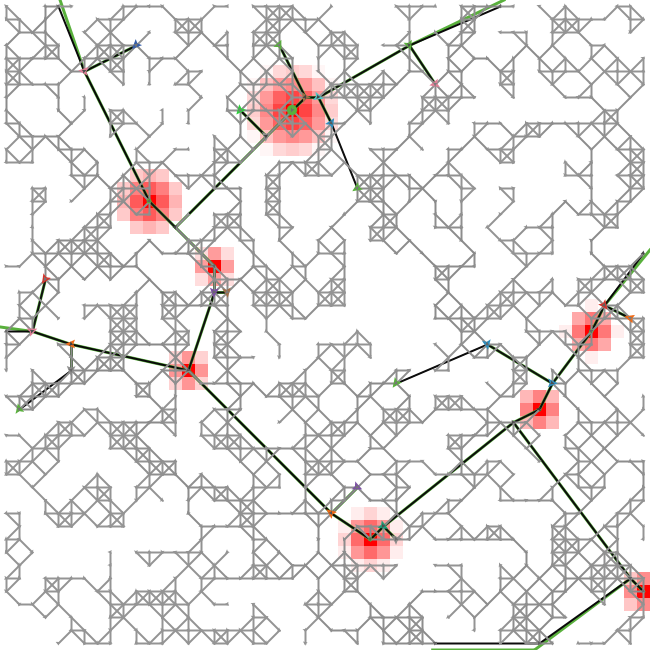
\includegraphics[width=0.48\linewidth]{Figures/NetworkGrowth/example-bio-process-1}}\hspace{0.2cm}
%\frame{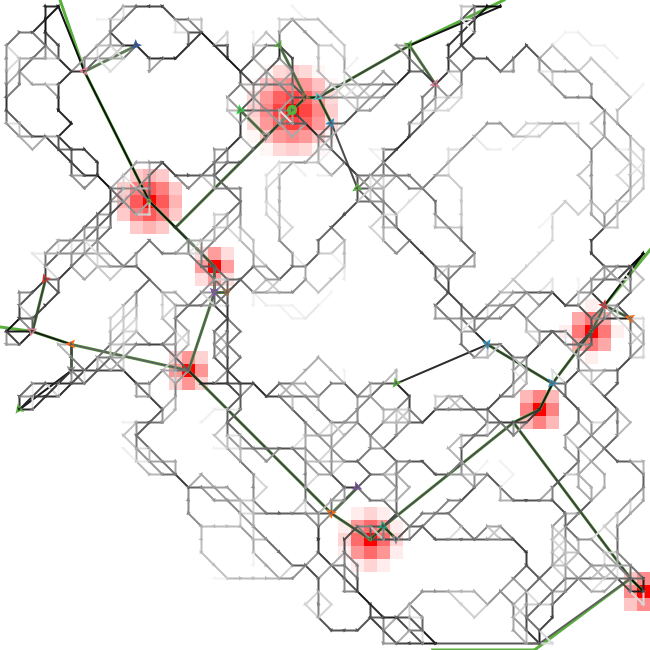
\includegraphics[width=0.48\linewidth]{Figures/NetworkGrowth/example-bio-process-1-tick80}}
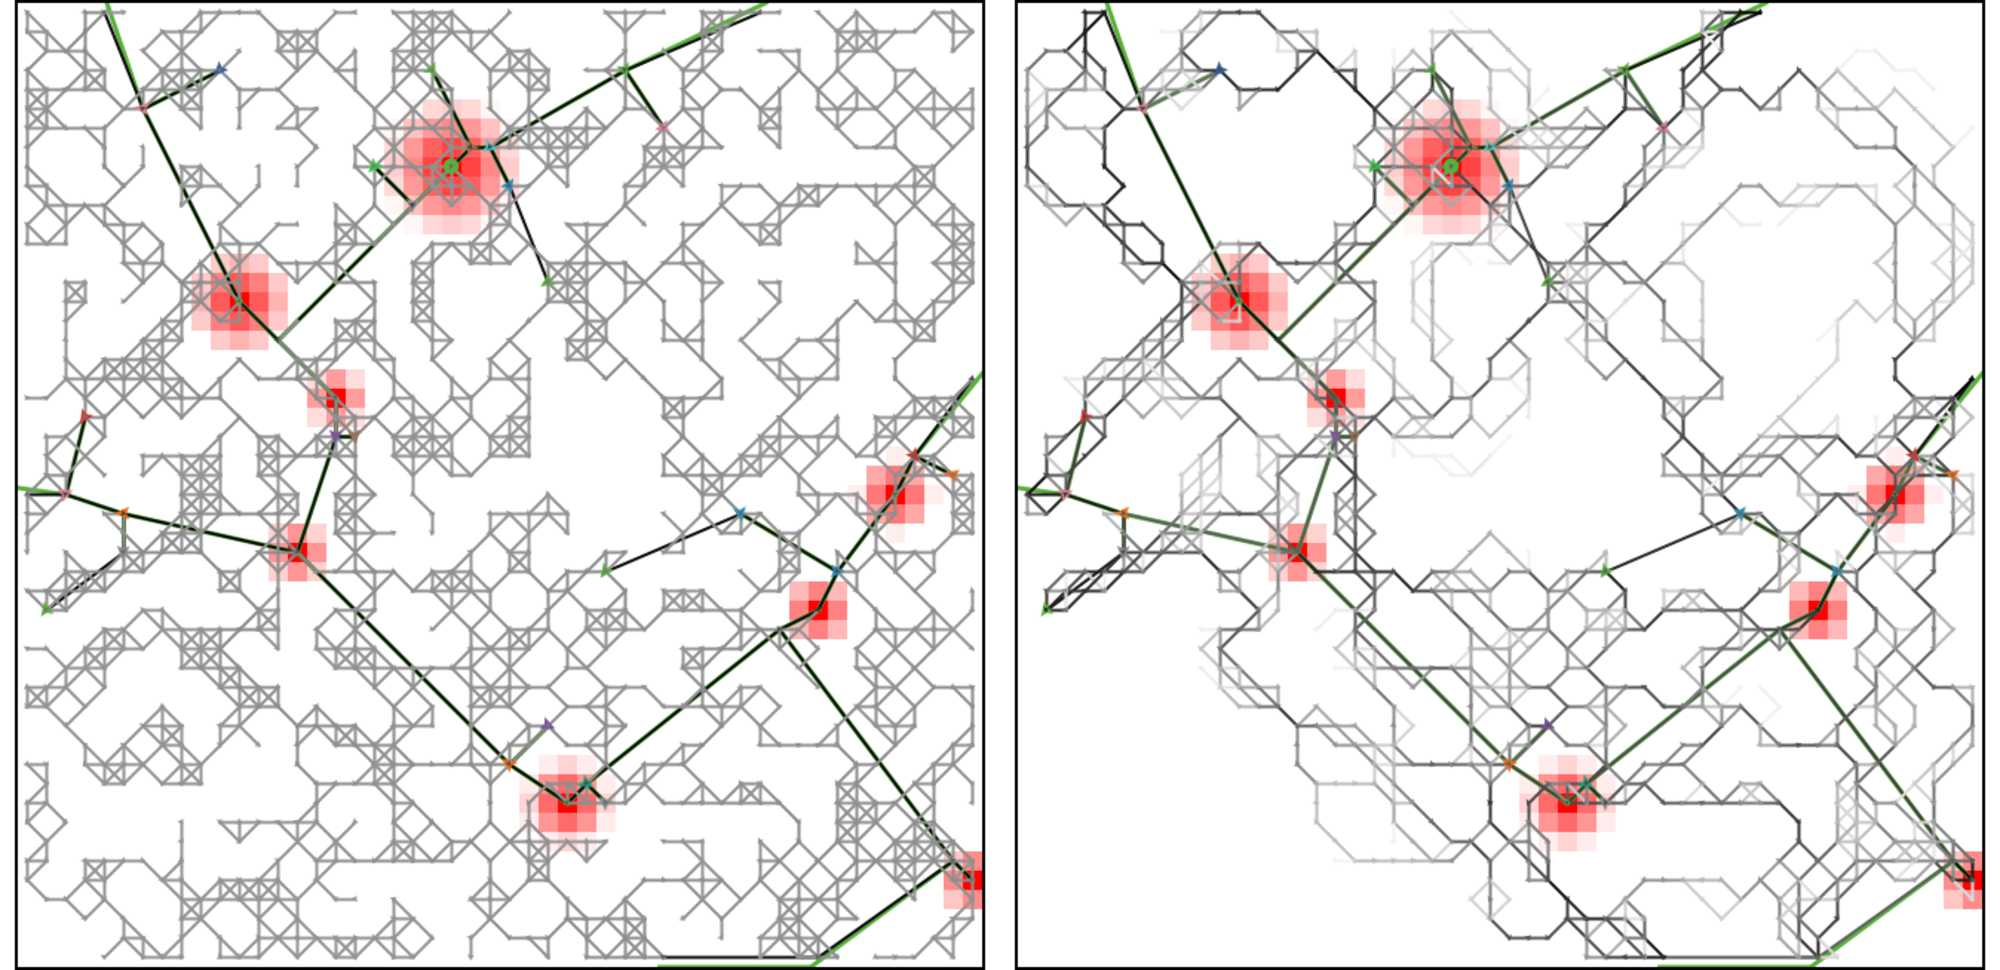
\includegraphics[width=\linewidth]{Figures/Final/7-1-1-fig-networkgrowth-bioexample.jpg}
\caption[Biological Network Example][Exemple du réseau biologique]{}{\textbf{Heuristique biologique pour la generation de réseau.} Cet exemple de visualisation illustre les étapes intermédiaires pour l'ajout de lien. \textit{(Gauche)} le réseau semi-aléatoire initial dans lequel le slime mould est lancé ; \textit{(Droite)} Même réseau après 80 itérations du slime mould, l'épaisseur des liens donnant la capacité.\label{fig:networkgrowth:bioexample}}
\end{figure}
%%%%%%%%%%%%%%%%%


%%%%%%%%%%%%%%%%%%%%%%%
\subsubsection{Cost-benefits}{Coûts-bénéfices}

La notion de cout n'est pas présente de manière explicite dans l'ensemble des heuristiques de croissance presentees jusqu'ici - elle l'est de manière implicite dans les potentiels de gravité par le paramètre d'attenuation de la distance, ainsi que dans le slime-mould puisque celui-ci génère des réseau compromis entre robustesse et cout. Nous ajoutons donc une heuristique simple qui est centrée sur le cout des tronçons de réseau lors de leur extension. Il s'agit de celle étudiée par~\cite{louf2013emergence}, qui se base sur des arguments d'économie des transports. Suivant une logique d'analyse coûts-bénéfices par les acteurs du développement du réseau, les liens sont réalisés séquentiellement pour les couples de villes non-connectées ayant un coût minimal, avec un coût de la forme $d_{ij} - \lambda / d_{ij}^2$.






%%%%%%%%%%%%%%%%%%%%%%%
\subsection{Results}{Résultats}


\subsubsection{Generated networks}{Réseaux générés}

Une illustration visuelle des différentes topologies générées est donnée en Fig~\ref{fig:networkgrowth:examples}. Les particularité de chacune des heuristiques sont immédiatement visibles. On voit par exemple




%%%%%%%%%%%%%%%%%
\begin{figure}
	%\frame{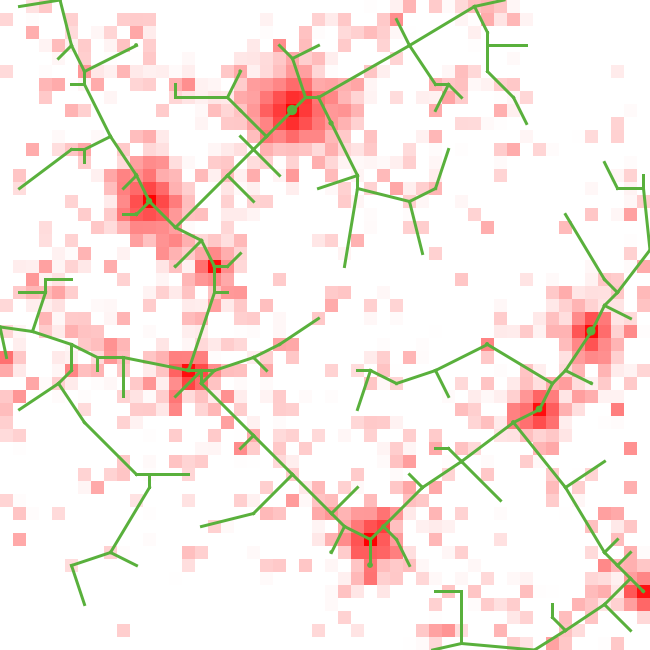
\includegraphics[width=0.32\linewidth]{Figures/NetworkGrowth/example_nw-connection}}
	%\frame{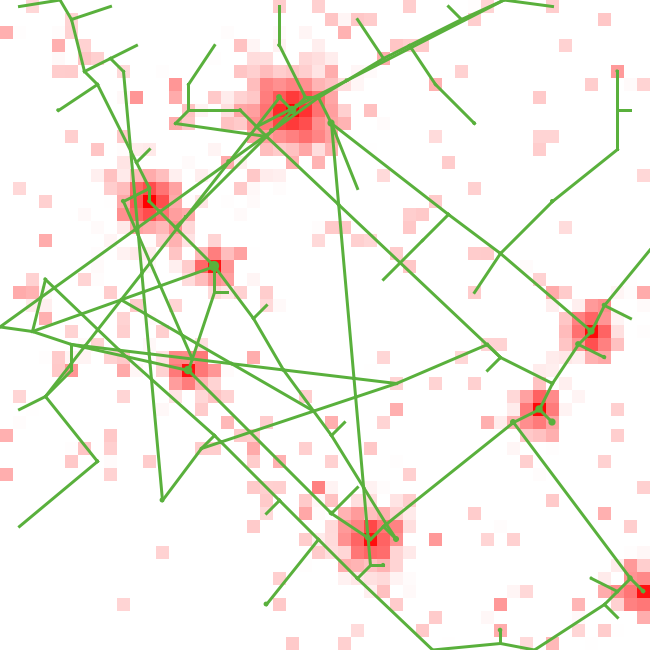
\includegraphics[width=0.32\linewidth]{Figures/NetworkGrowth/example_nw-random}}
	%\frame{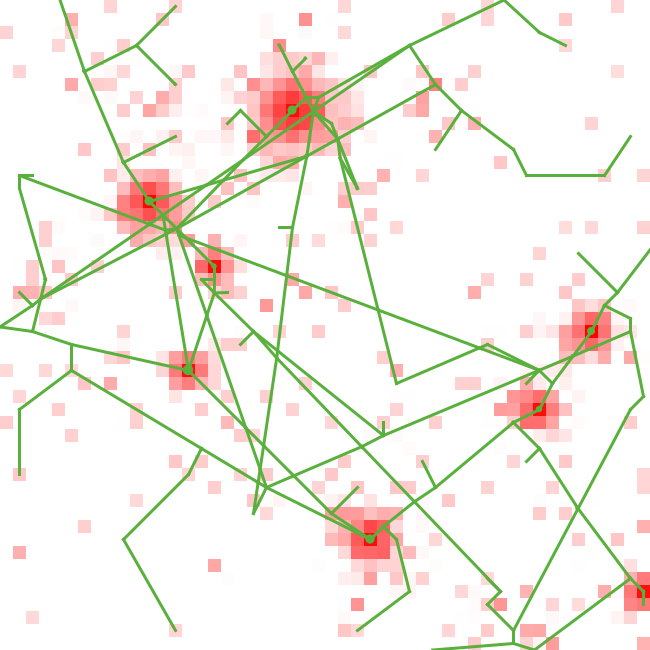
\includegraphics[width=0.32\linewidth]{Figures/NetworkGrowth/example_nw-rndbrkdwn}}\\
	%\frame{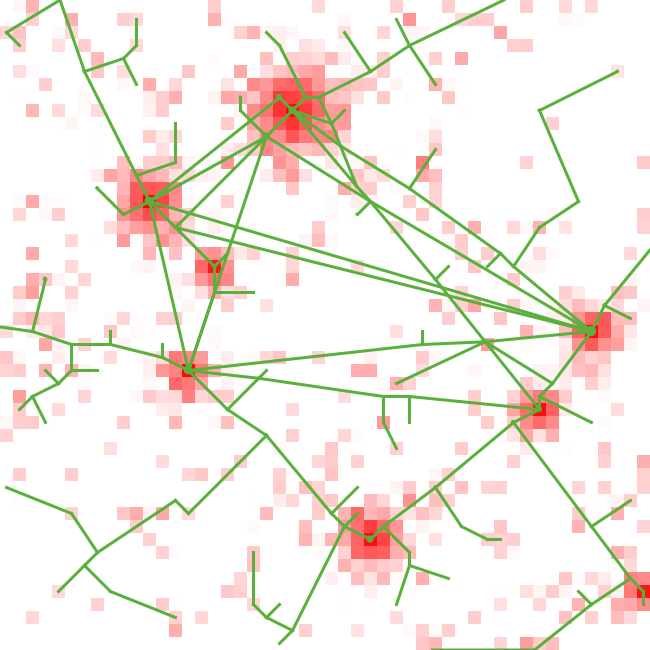
\includegraphics[width=0.32\linewidth]{Figures/NetworkGrowth/example_nw-gravity}}
	%\frame{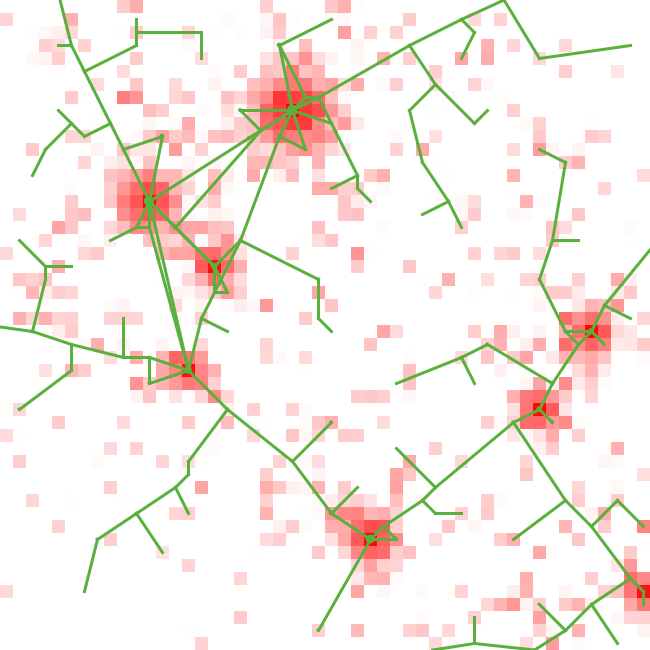
\includegraphics[width=0.32\linewidth]{Figures/NetworkGrowth/example_nw-cost}}
	%\frame{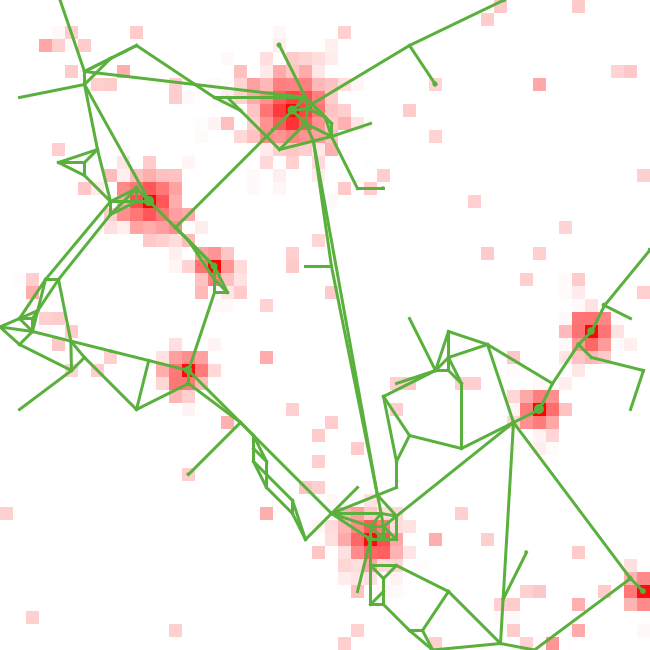
\includegraphics[width=0.32\linewidth]{Figures/NetworkGrowth/example_nw-bio}}
	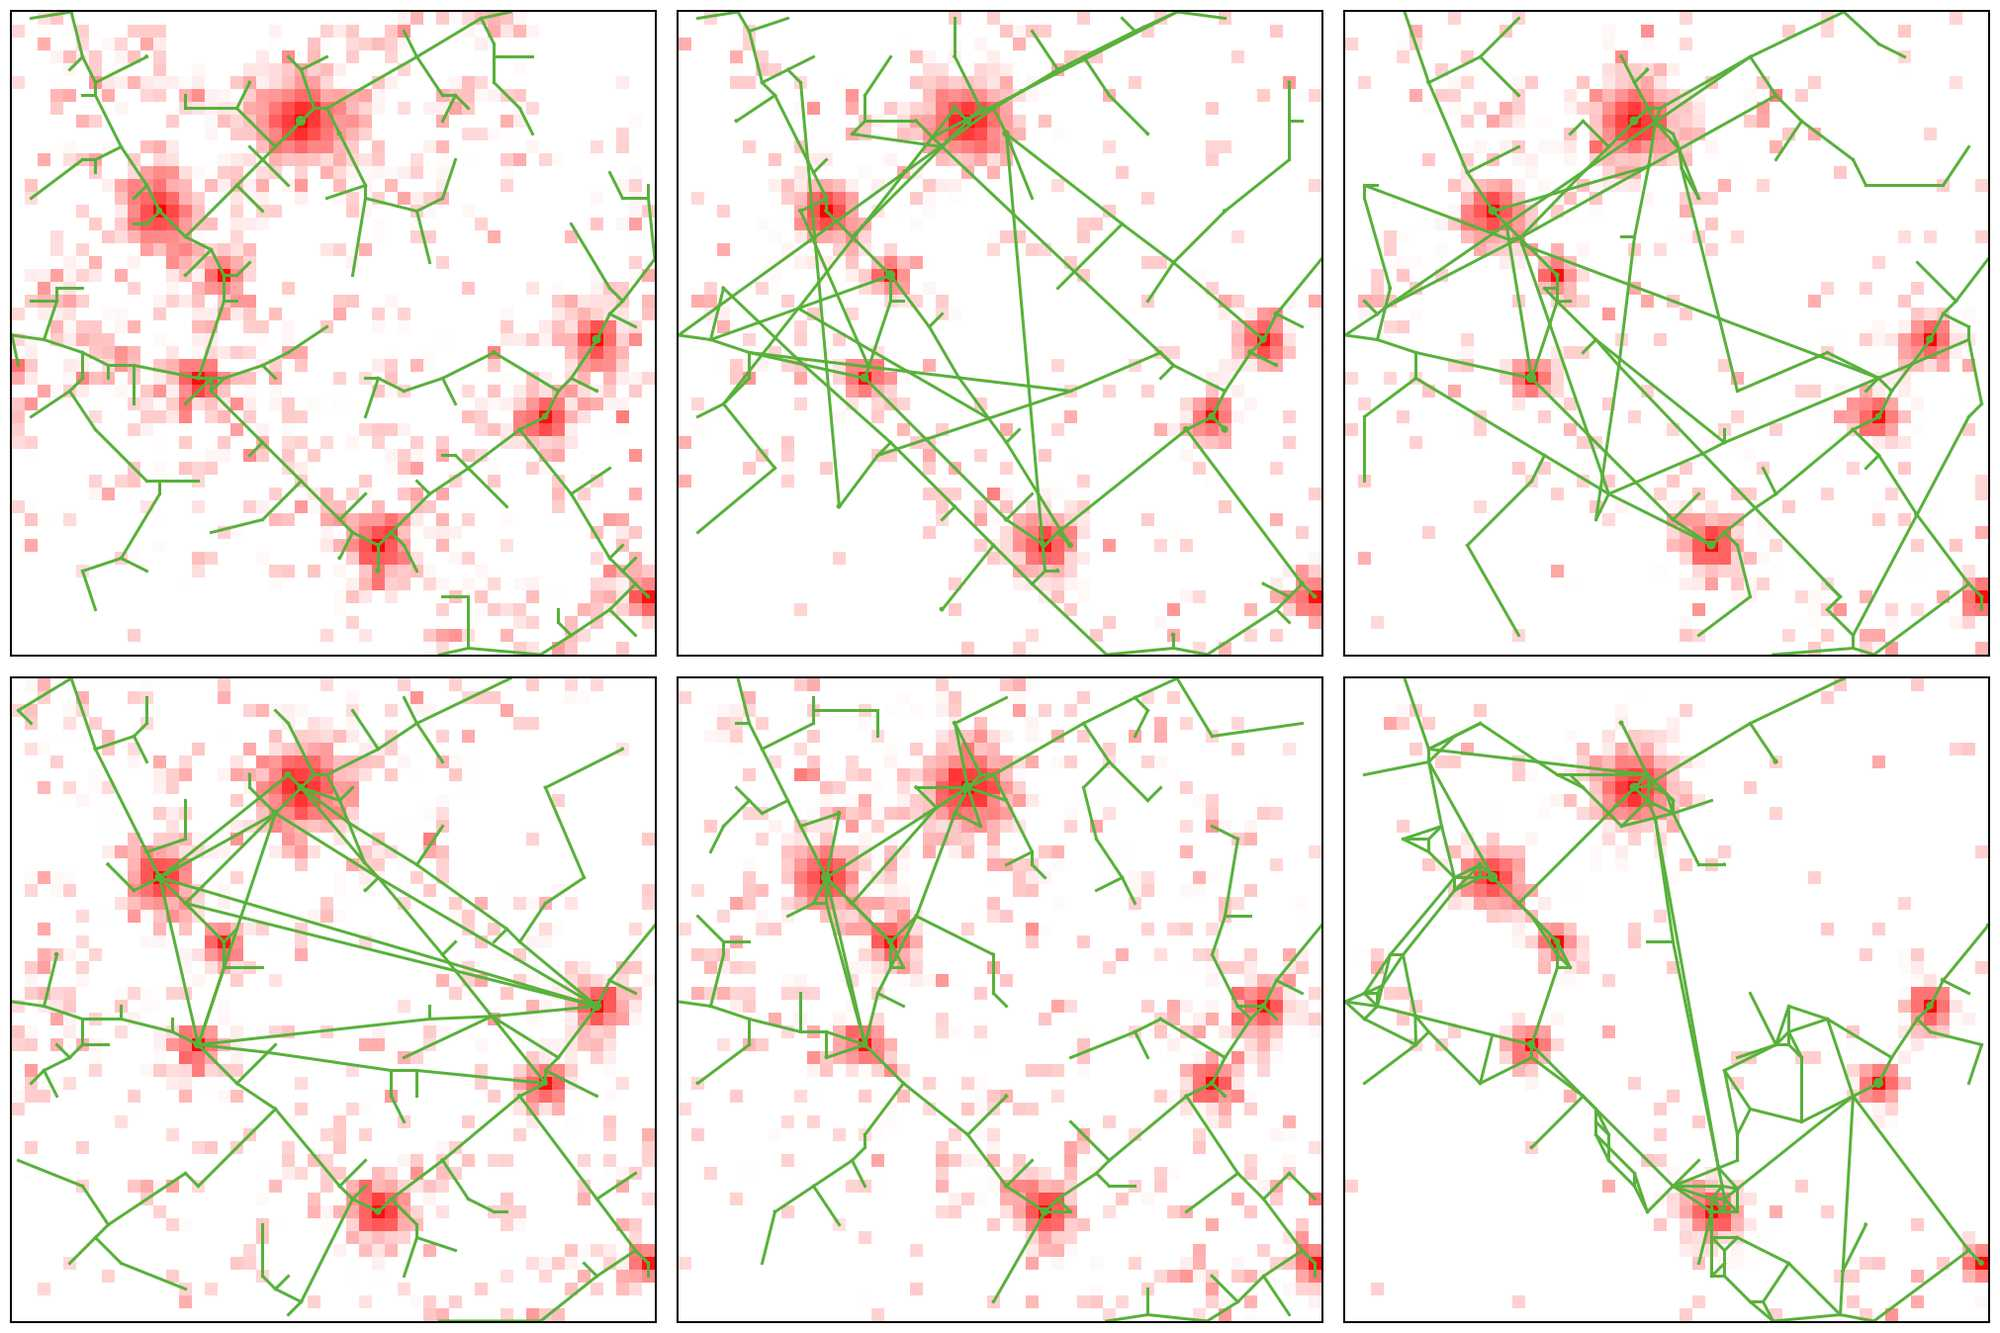
\includegraphics[width=\linewidth]{Figures/Final/7-1-2-fig-networkgrowth-examples.jpg}
\caption[Network examples][Exemples de réseaux]{\label{fig:networkgrowth:examples}}{\textbf{Exemples de réseaux obtenus par les différentes heuristiques}\label{fig:networkgrowth:examples}}
\end{figure}
%%%%%%%%%%%%%%%%%




\subsubsection{Experience plan}{Plan d'expérience}



La longueur de réseau finale n'est pas directement contrôlée par les paramètres, nous fixons un critère d'arrêt de croissance du réseau à nombre de lien fixe pour pouvoir comparer les réseaux finaux. La génération de réseau est faite à densité de population constante, sur configurations réelles classifiées morphologiquement en~\ref{sec:staticcorrelations}. 


\subsubsection{Feasible space}{Topologies obtenues}

Les réseaux sont caractérisés par les indicateurs suivants : centralité de chemin et de proximité moyennes, diamètre, longueur moyenne de chemin, vitesse relative. Pour visualiser les espaces faisables et les comparer aux réseaux réels par la suite, 





%%%%%%%%%%%%%%%%%
\begin{figure}
%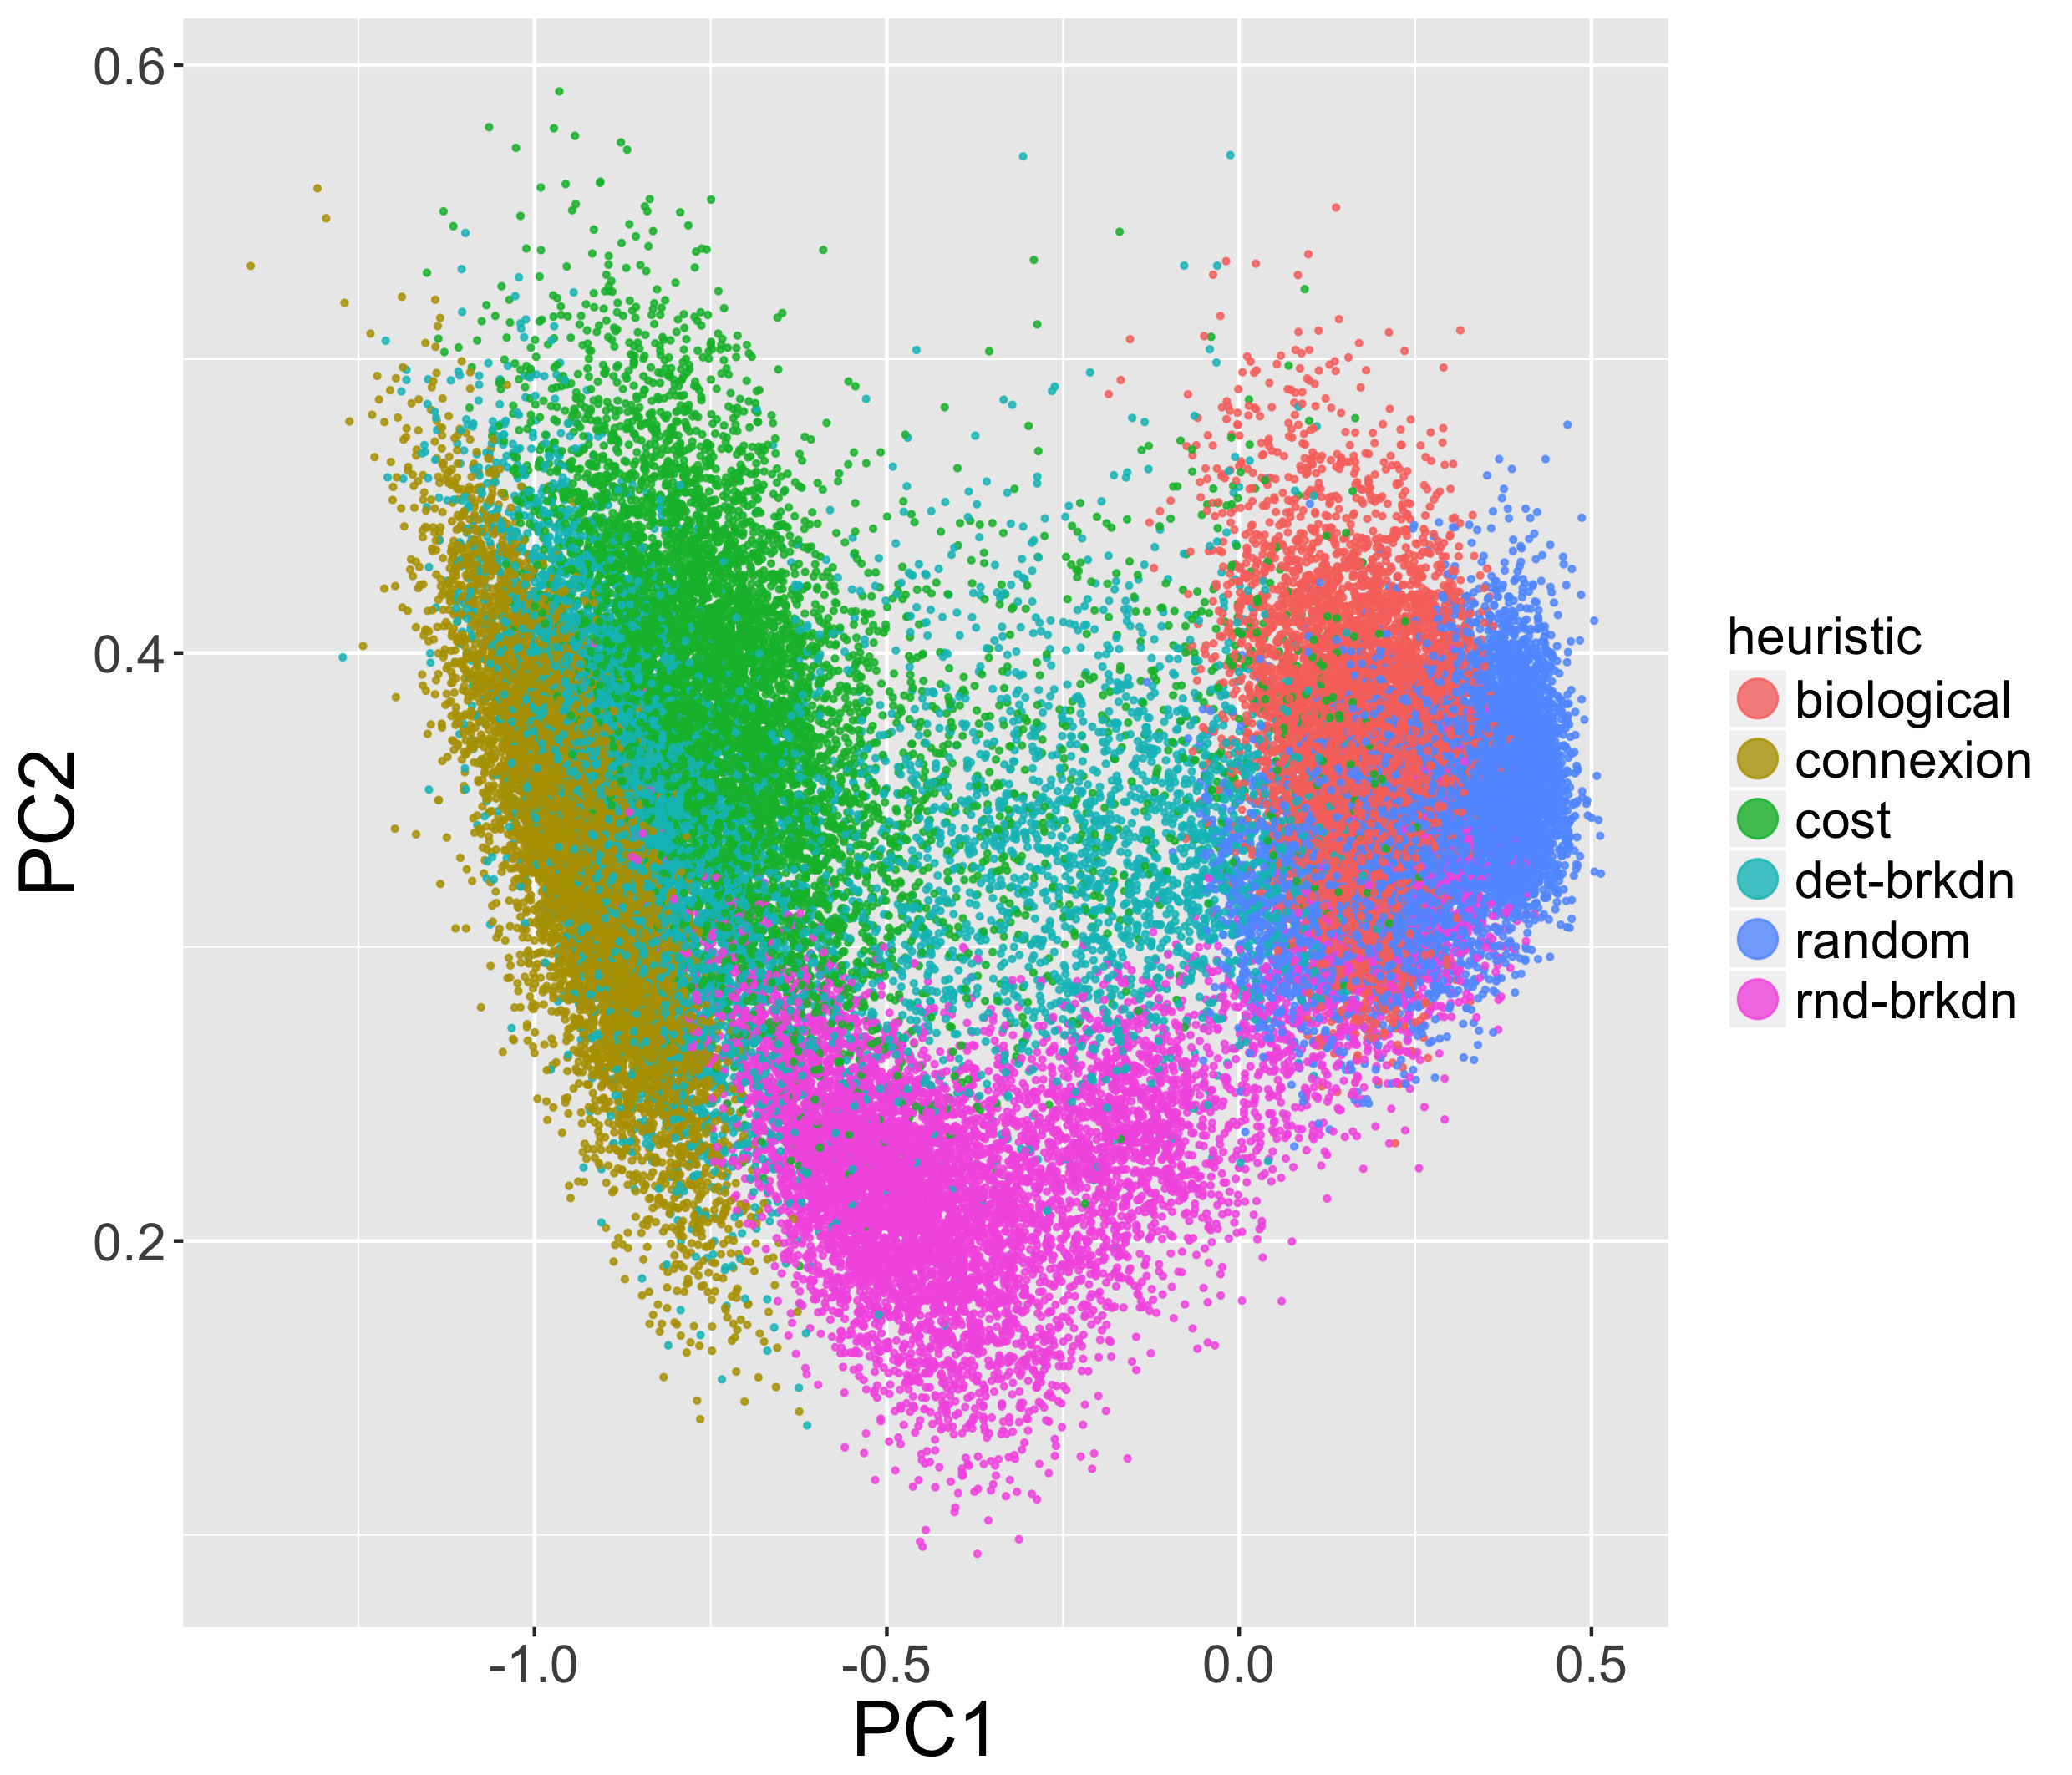
\includegraphics[width=\linewidth]{Figures/NetworkGrowth/feasible_space_pca}
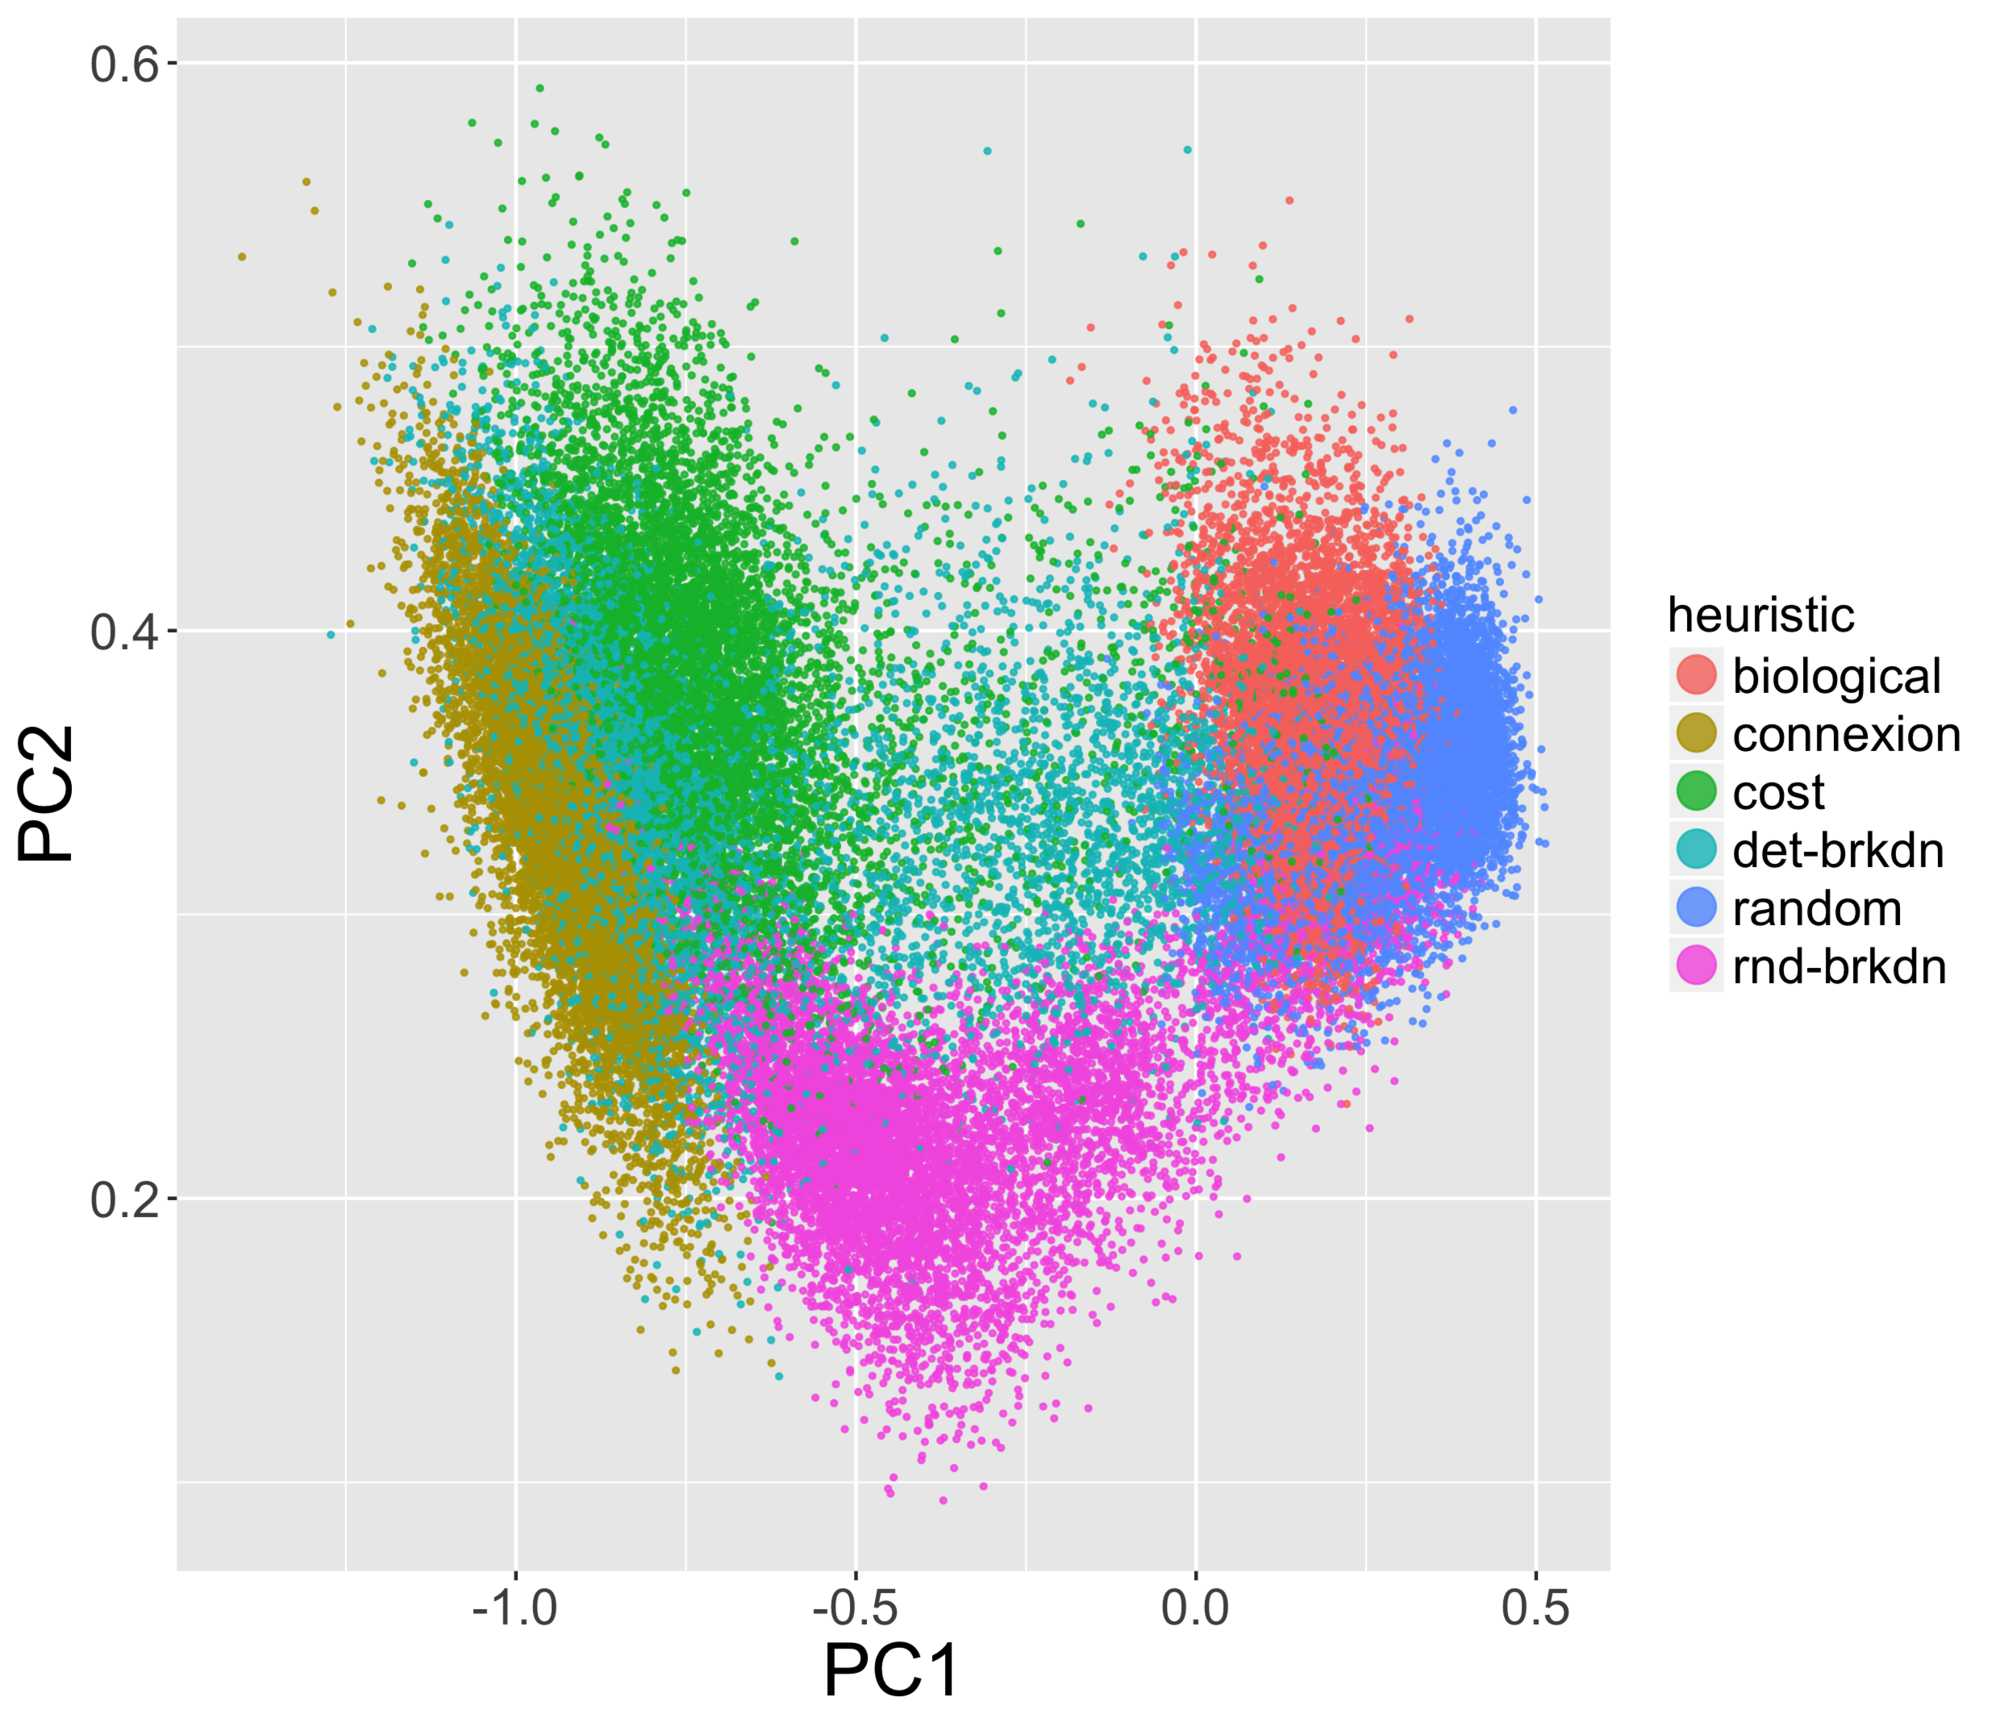
\includegraphics[width=\linewidth]{Figures/Final/7-1-2-fig-networkgrowth-feasiblespace.jpg}
\caption[Feasible topological space][Espace topologique faisable]{}{\textbf{Espace topologique faisable pour les différentes heuristiques de génération.} La même figure conditionnée à la classe morphologique de densité est donnée en Appendice~\ref{app:sec:networkgrowth}.\label{fig:networkgrowth:feasiblespace}}
\end{figure}
%%%%%%%%%%%%%%%%%

% PCA synth
%
%                                PC1        PC2        PC3        PC4         PC5
%meanBwCentrality        -0.51420330 -0.4500671  0.5415210 -0.4602950  0.16708710
%meanPathLength          -0.45662839  0.1782617 -0.2556133  0.3151101  0.77141477
%meanRelativeSpeed        0.57854267  0.3344679  0.3147784 -0.4083421  0.53627500
%nwDiameter              -0.43570261  0.8011179  0.1305644 -0.2508956 -0.29728372
%meanClosenessCentrality  0.05036956  0.1095611  0.7247651  0.6776003 -0.03213514
%Importance of components:
%                          PC1     PC2     PC3     PC4     PC5
%Standard deviation     0.4981 0.06762 0.04611 0.03423 0.02982
%Proportion of Variance 0.9659 0.01780 0.00828 0.00456 0.00346
%Cumulative Proportion  0.9659 0.98370 0.99198 0.99654 1.00000



\subsubsection{Real network comparison}{Comparaison aux réseaux réels}


Nous utilisons les mesures sur réseaux routiers réels calculées en~\ref{sec:staticcorrelations} pour calculer une distance des configurations générées aux configurations réelles. Nous prenons une distance euclidienne simple sur les vecteurs d'indicateurs.




%%%%%%%%%%%%%%%%%
\begin{figure}
%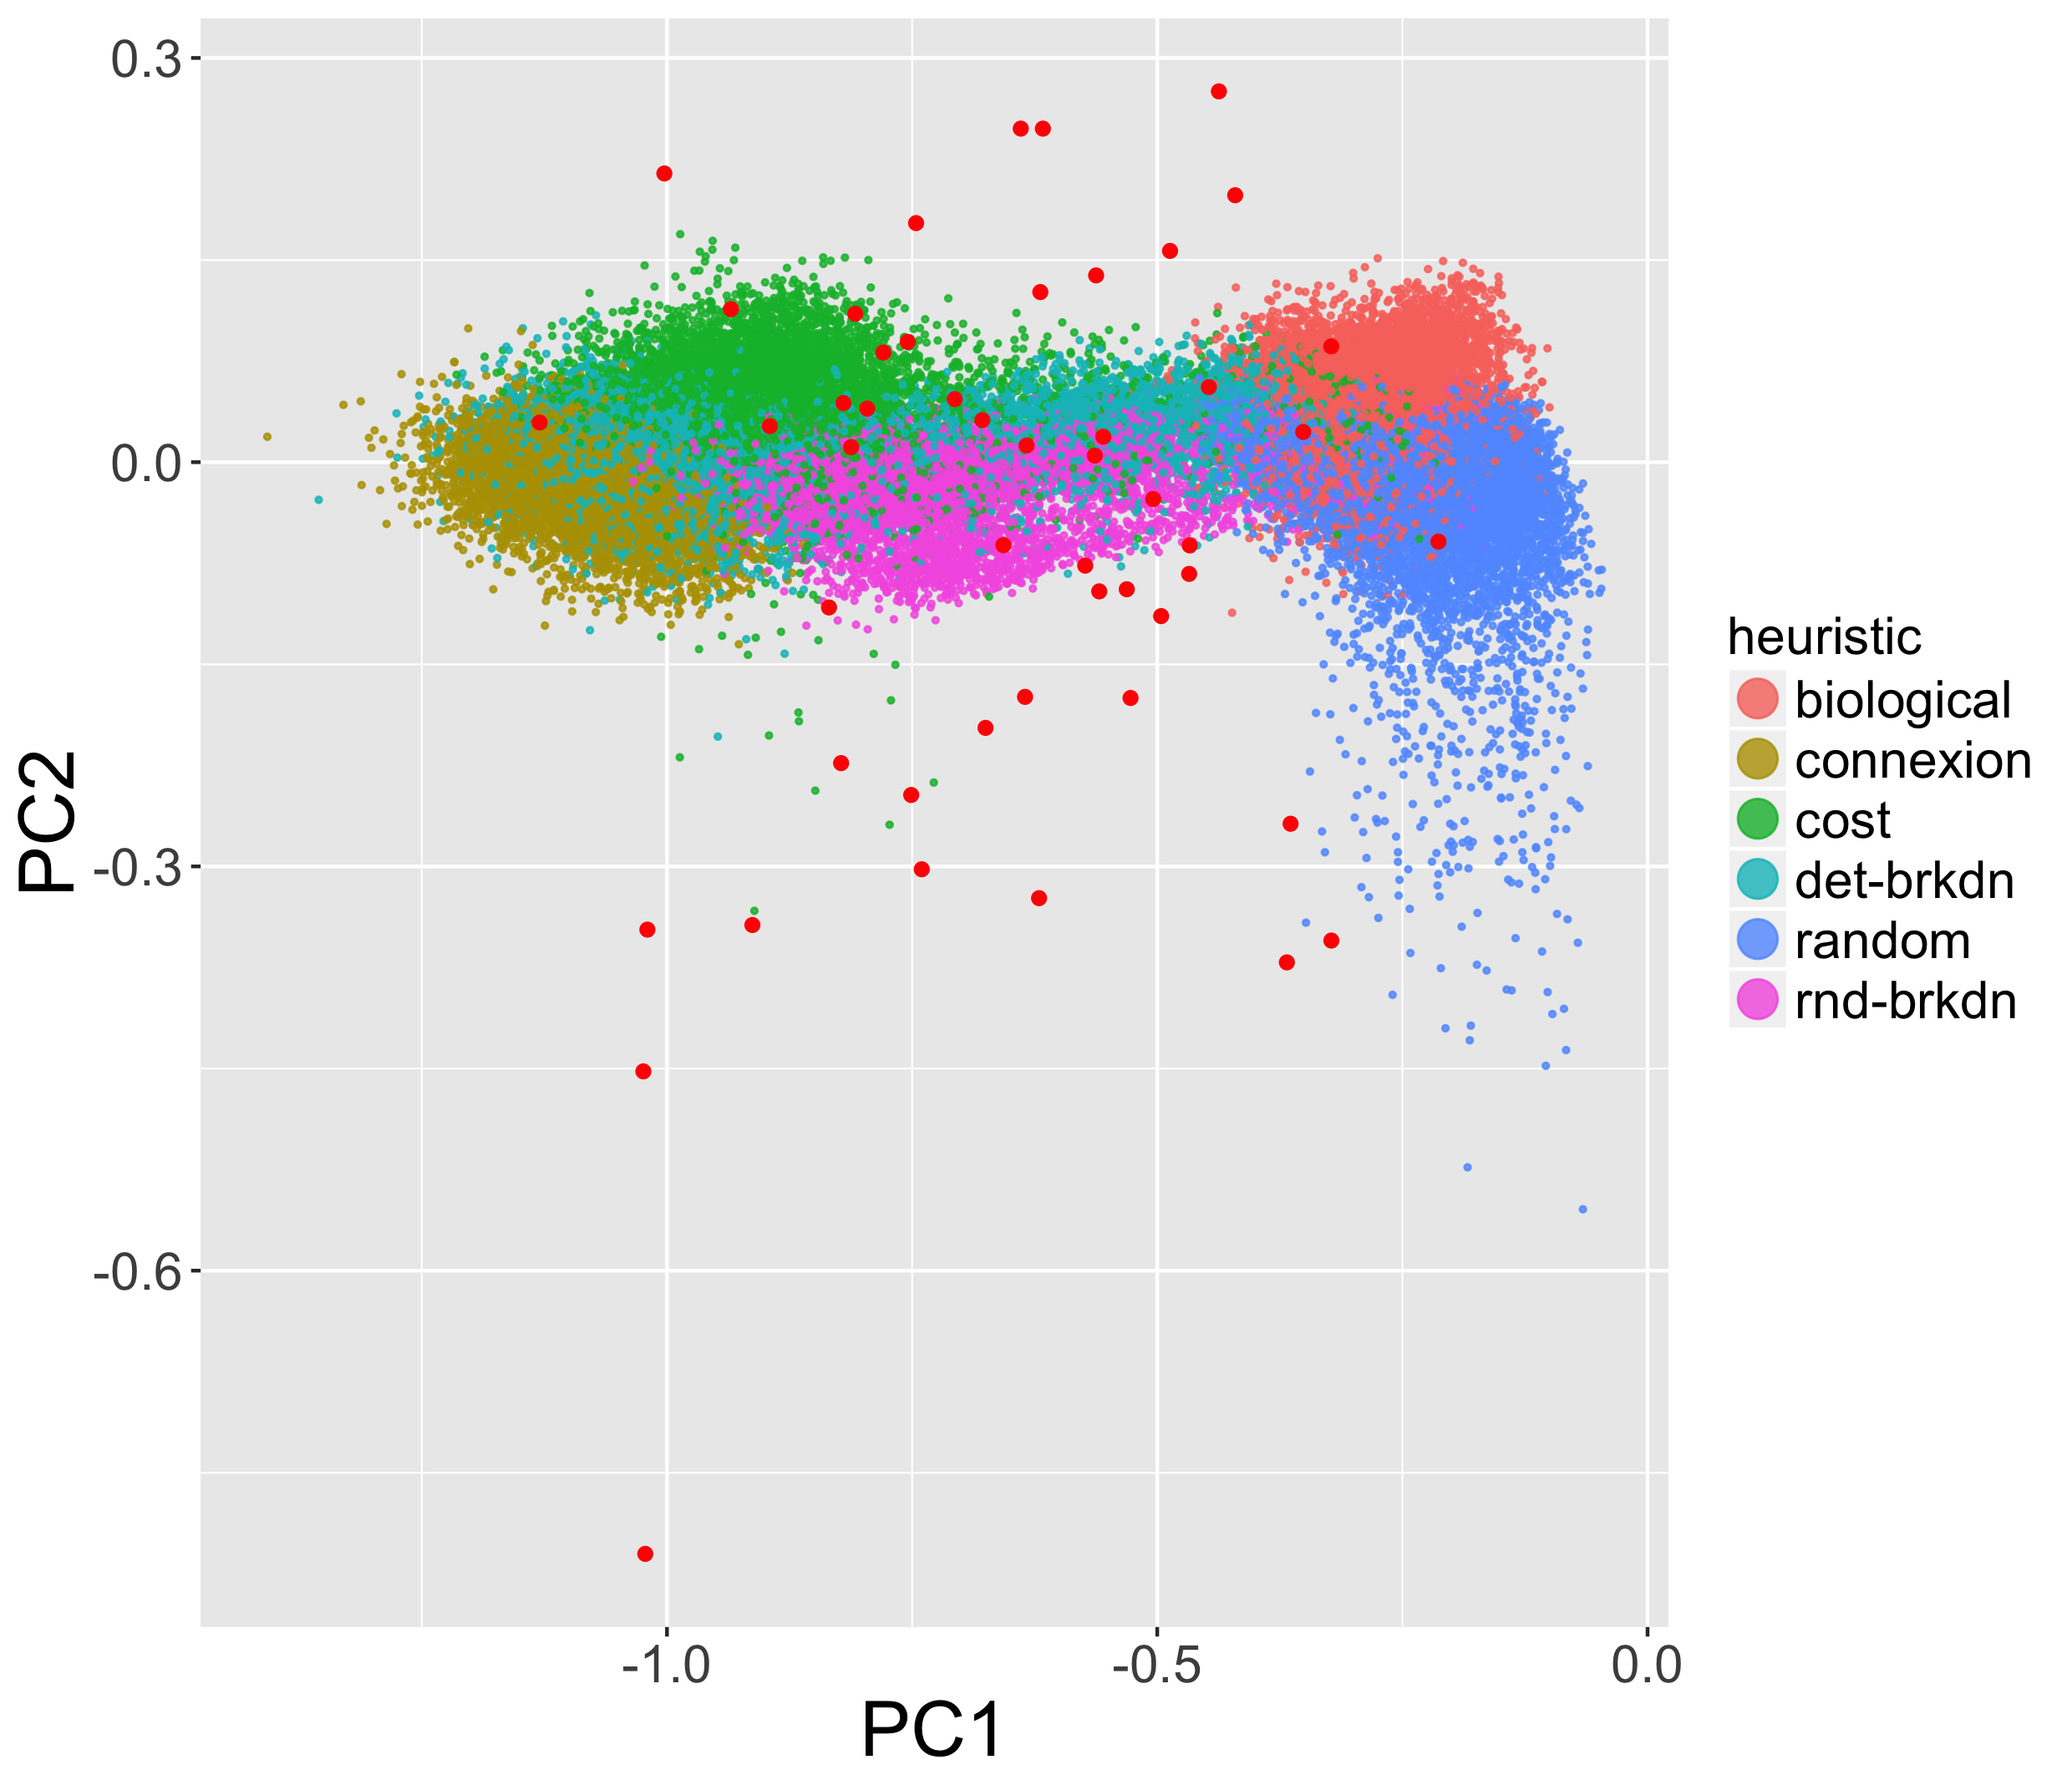
\includegraphics[width=0.45\linewidth]{Figures/NetworkGrowth/feasible_space_withreal_pca}
%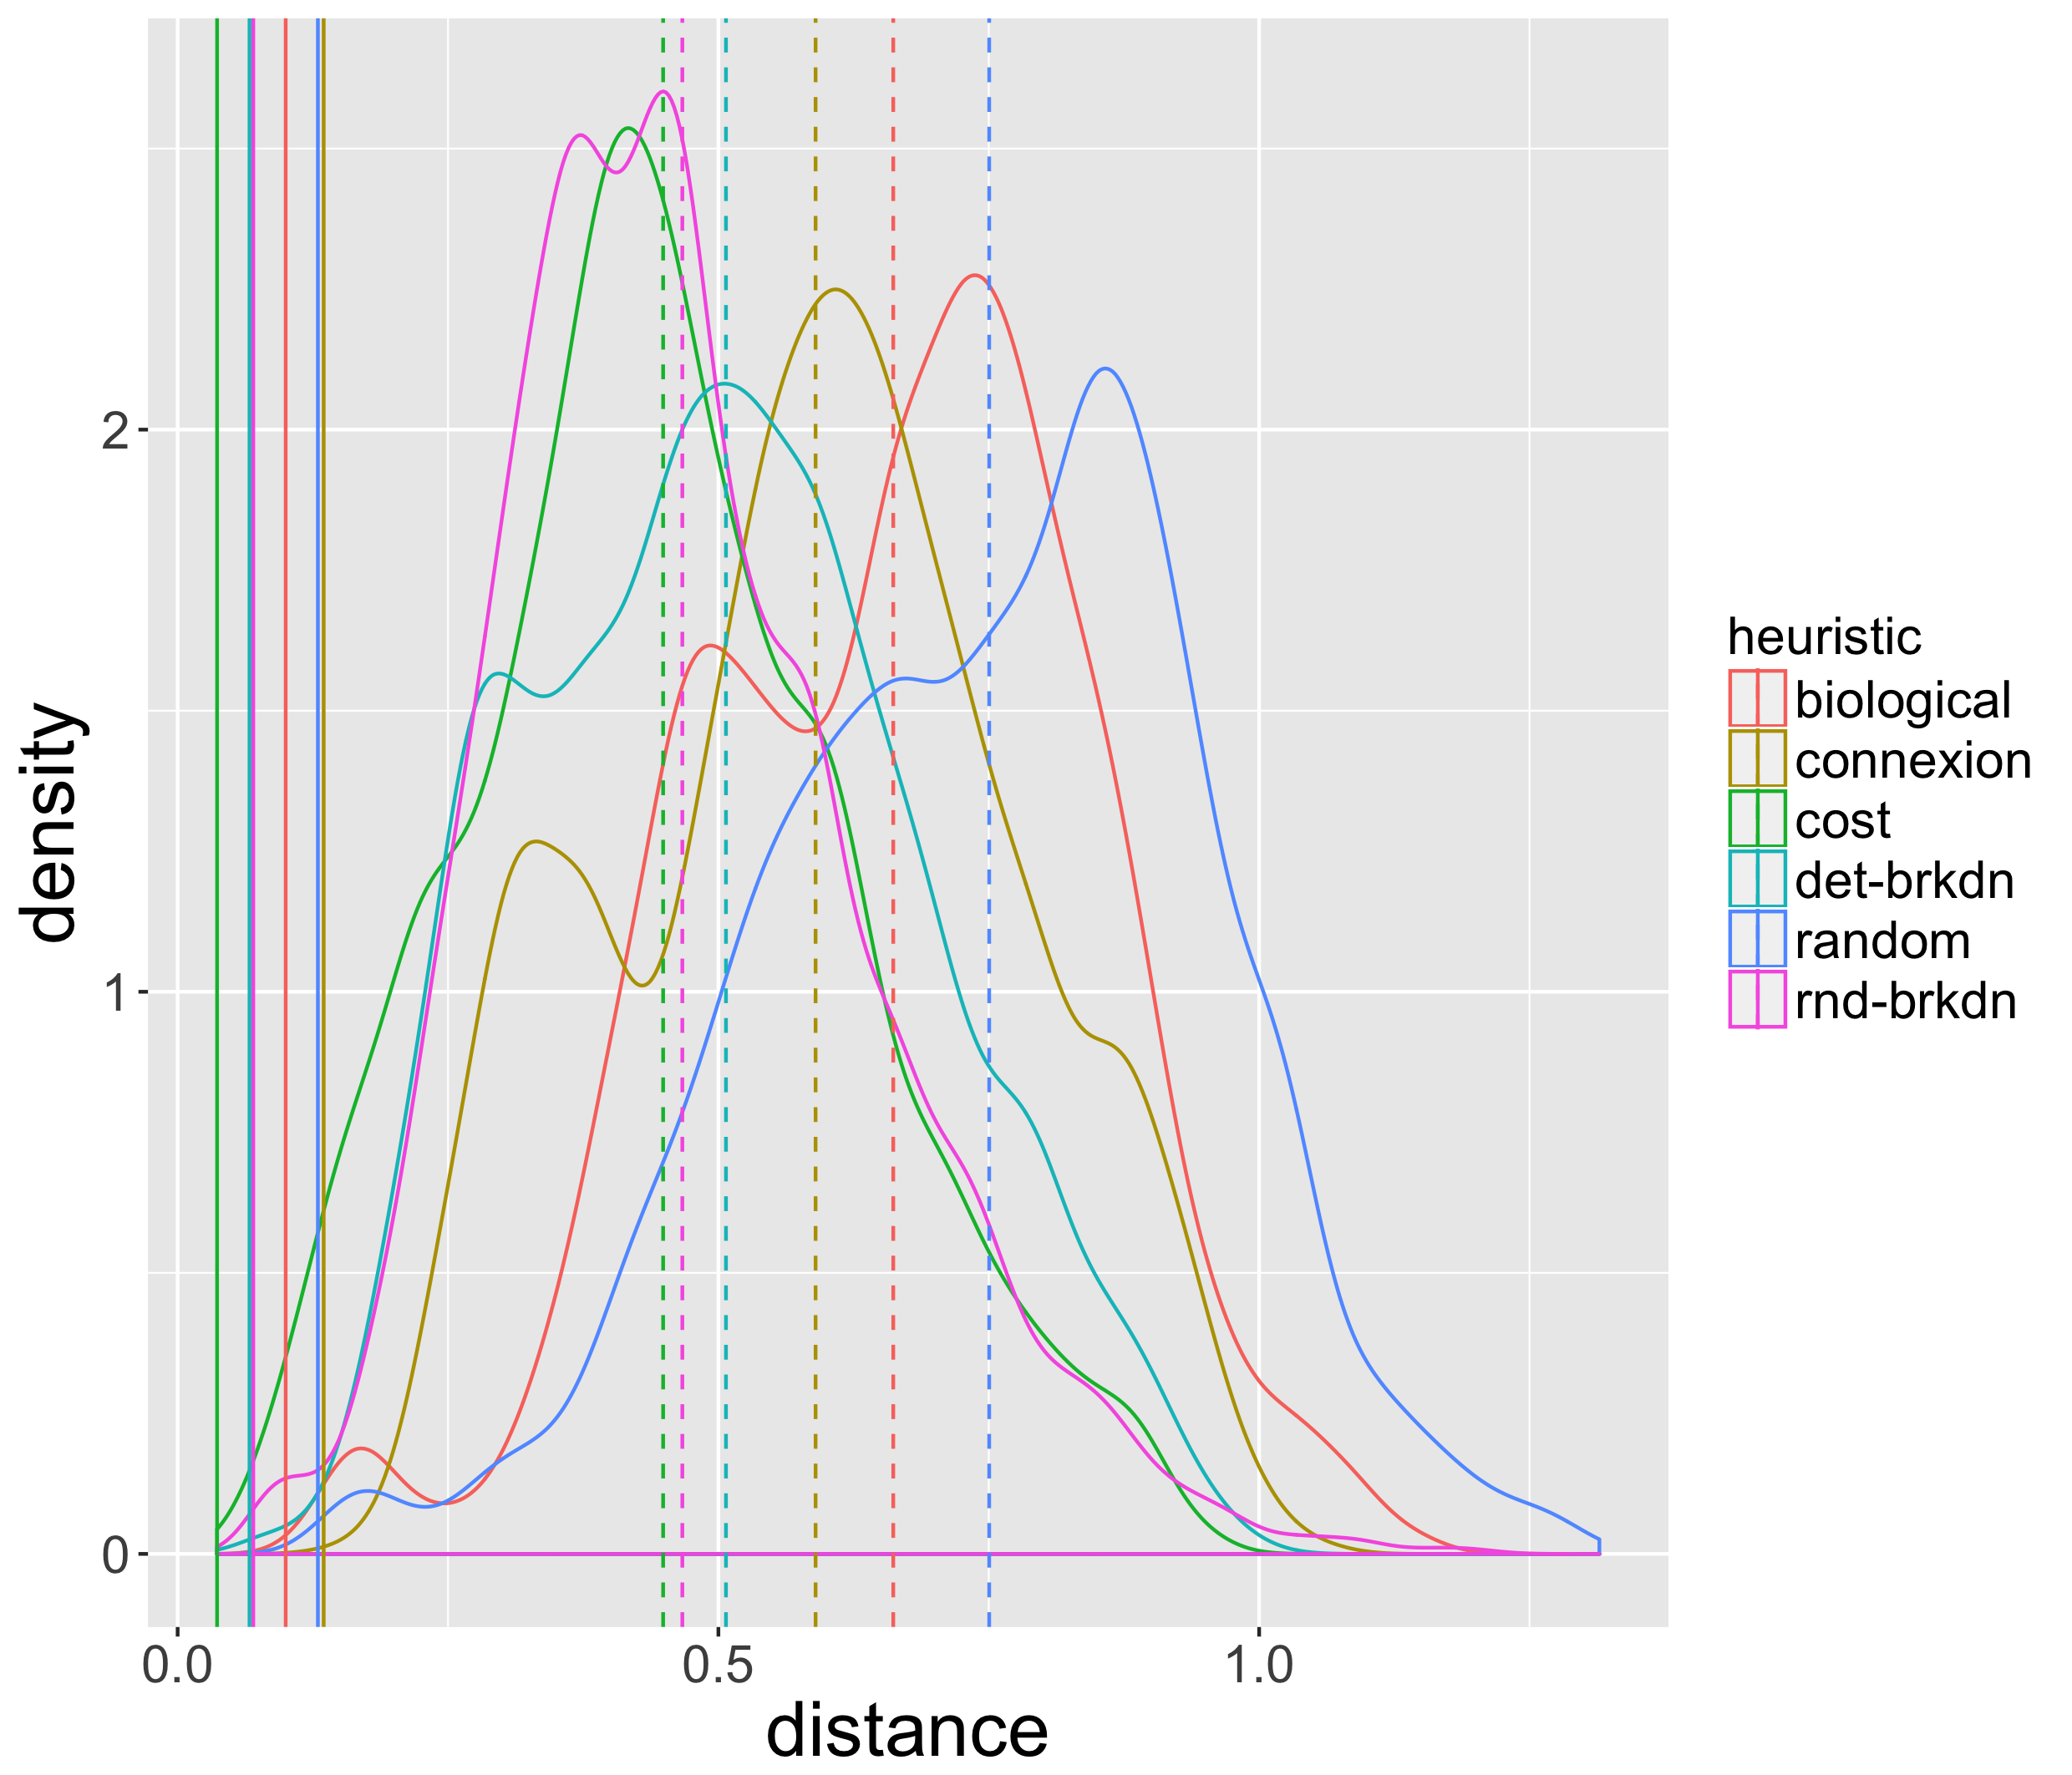
\includegraphics[width=0.45\linewidth]{Figures/NetworkGrowth/distance_real}\\
%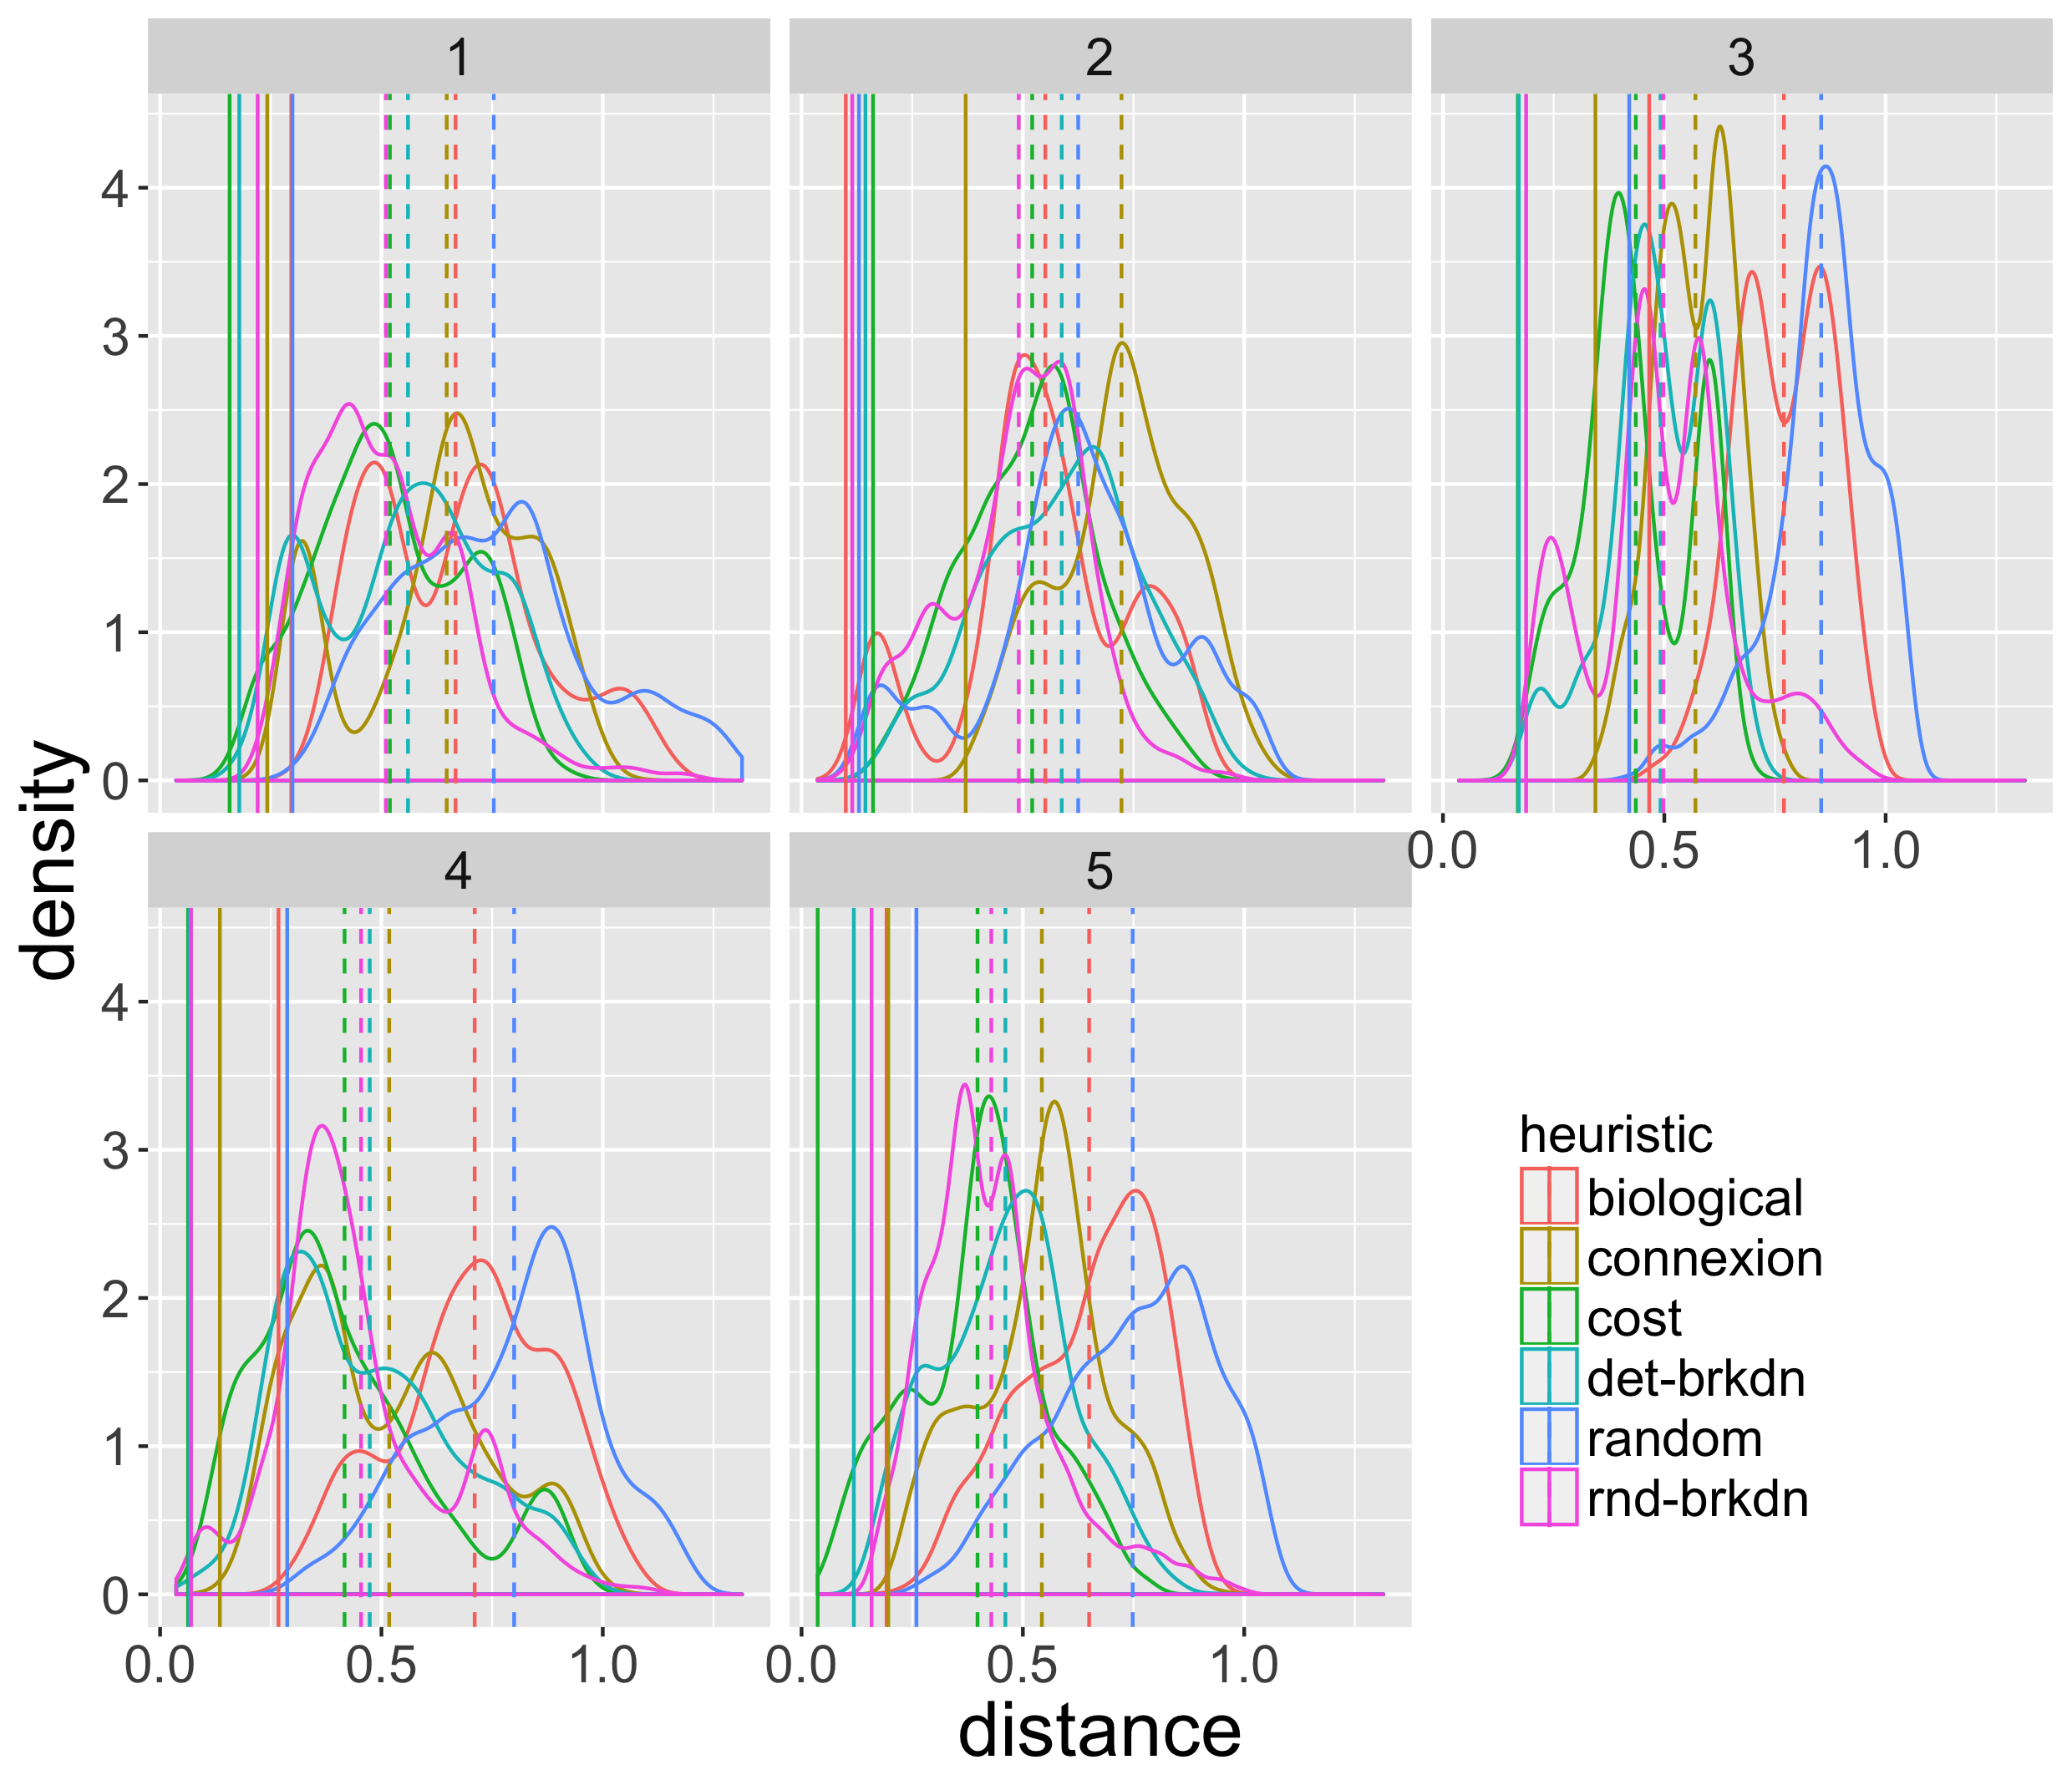
\includegraphics[width=0.8\linewidth]{Figures/NetworkGrowth/distance_real_bymorph}
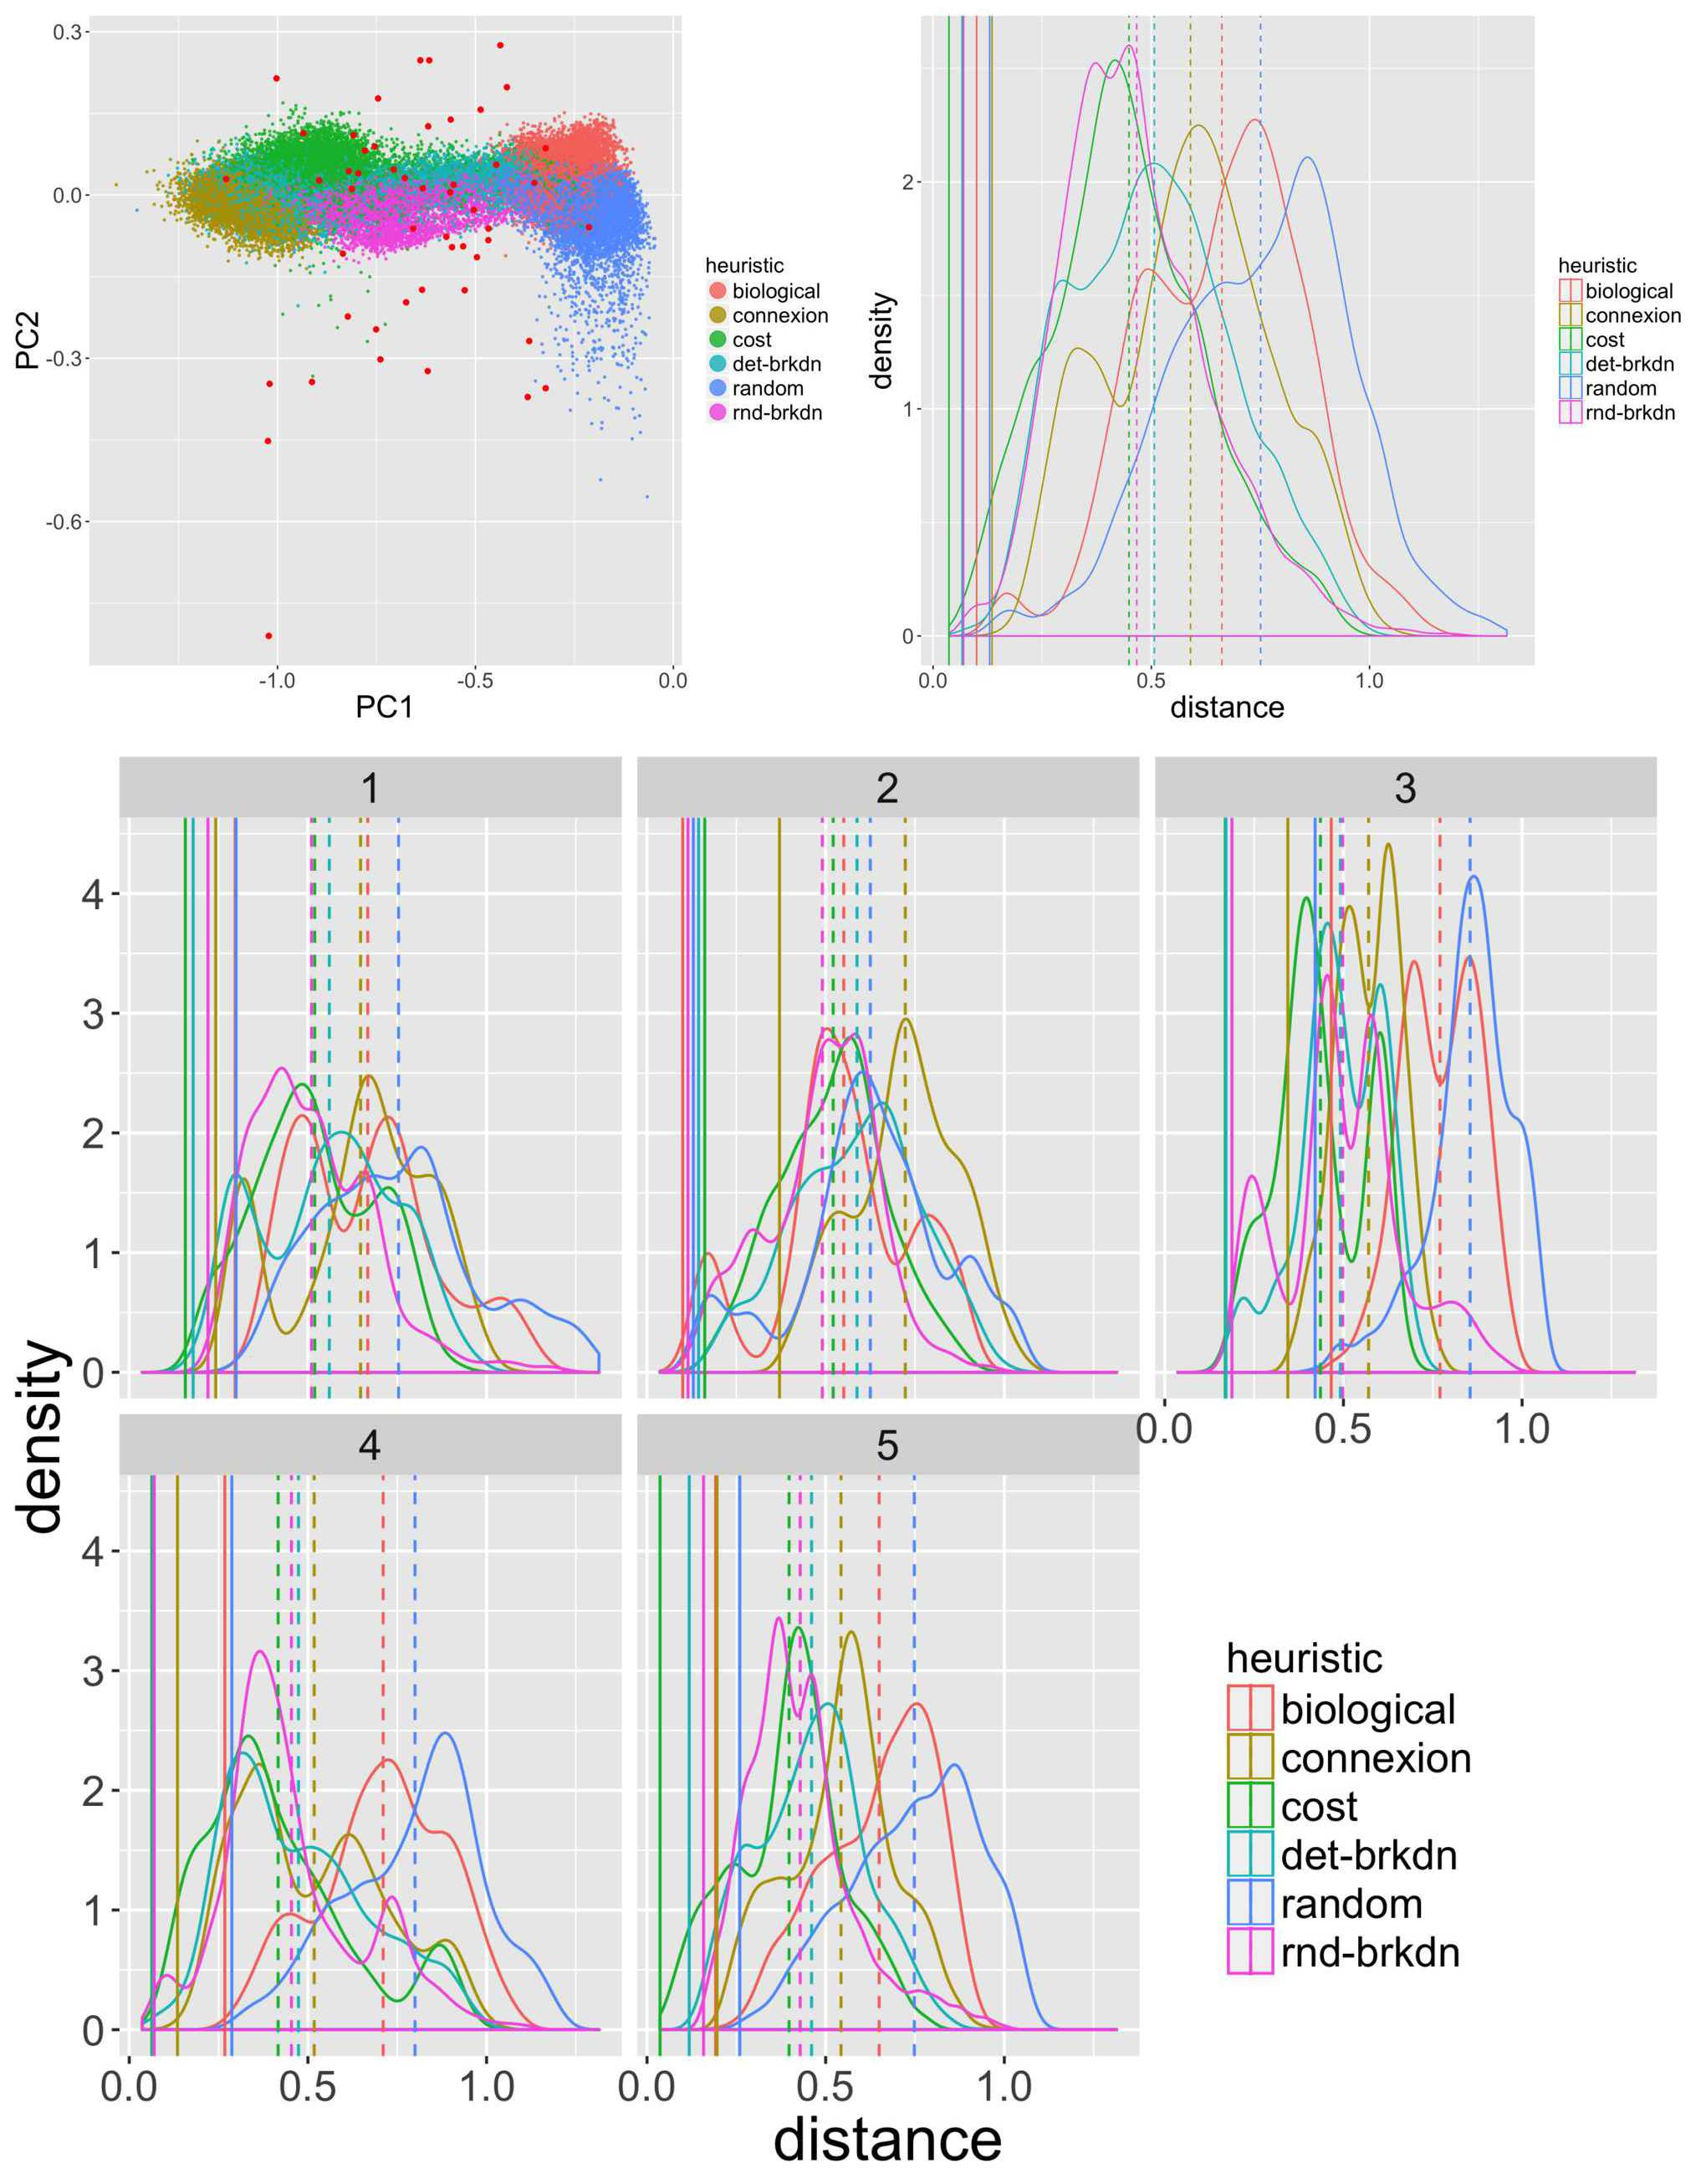
\includegraphics[width=\linewidth]{Figures/Final/7-1-2-fig-networkgrowth-realdistance}
\caption[][Comparaison aux réseaux réels]{}{\textbf{Comparaison aux réseaux réels.} \textit{(Haut Gauche)}\label{fig:networkgrowth:realdistance}}
\end{figure}
%%%%%%%%%%%%%%%%%



% PCA real

%Rotation:
%                        PC1        PC2          PC3         PC4         PC5
%meanBetweenness  0.32071179  0.9123552 -0.101287507  0.09905262 -0.21137945
%meanCloseness   -0.01926100  0.2063540 -0.009888761  0.19655887  0.95828695
%networkPerf     -0.05108717 -0.1222155  0.053354929  0.97433440 -0.17400925
%diameter         0.66374922 -0.1381554  0.733028737 -0.01314015  0.05335036
%Importance of components:
%                          PC1     PC2     PC3     PC4     PC5
%Standard deviation     0.1084 0.08207 0.05094 0.03375 0.02602
%Proportion of Variance 0.5132 0.29415 0.11332 0.04976 0.02957
%Cumulative Proportion  0.5132 0.80736 0.92067 0.97043 1.00000
%


% Distances

%nres%>%group_by(heuristic)%>%summarise(distance=min(distance))
%1 biological 0.09990225
%2  connexion 0.13504050
%3       cost 0.03647362
%4  det-brkdn 0.06644744
%5     random 0.12968739
%6  rnd-brkdn 0.06994303
%
%nres%>%group_by(heuristic)%>%summarise(distance=mean(distance))
%
%1 biological 0.6616921
%2  connexion 0.5898689
%3       cost 0.4489075
%4  det-brkdn 0.5070177
%5     random 0.7504109
%6  rnd-brkdn 0.4666547
%
%nres%>%group_by(heuristic)%>%summarise(distance=median(distance))
%
%1 biological 0.6780299
%2  connexion 0.5973273
%3       cost 0.4359749
%4  det-brkdn 0.5024551
%5     random 0.7680822
%6  rnd-brkdn 0.4462033


%%%%%%%%%%%%%%%%%%%%%%%
\subsection{Discussion}{Discussion}



Si le modèle slime-mould a été montré comme traduisant de manière simplifiée une génération de réseaux robustes, son utilisation pour la planification a été mise en question, notamment pour sa non prise en compte de facteurs extérieurs et de l'environnement urbain~\cite{adamatzky2010road}. Nos résultats semblent confirmer ces analyses, puisque cette heuristique est la moins performante au sens de la distance aux réseaux réels.










